\documentclass[a4paper,11pt]{article}
\usepackage[utf8]{inputenc}
\usepackage[T1]{fontenc}
\usepackage[english]{babel}
\usepackage{lmodern}\usepackage{microtype}
\usepackage{amsmath,amssymb,bm,mathtools}
\usepackage{geometry}
\geometry{a4paper,left=2.3cm,right=2.3cm,top=2.0cm,bottom=2.0cm}
\usepackage{booktabs,array}
\usepackage{xcolor}\definecolor{bokug}{RGB}{0,135,60}
\usepackage{tikz}
\usetikzlibrary{patterns,arrows.meta,calc,decorations.pathmorphing}
\usepackage{fancyhdr}\pagestyle{fancy}
\renewcommand{\headrulewidth}{0.4pt}
\usepackage{enumitem}\setlength{\parindent}{0pt}\setlength{\parskip}{4pt}

\begin{document}
\fancyhead[L]{\small VU Mechanik – LAWI 100515 (PI)}
\fancyhead[R]{\small SS 2026}
\fancyfoot[C]{\thepage}
\begin{center}{\large\bfseries\color{bokug}University of Natural Resources and Life Sciences, Vienna (BOKU)}\\[2pt]{\large\bfseries VU Mechanik – LAWI 100515 (PI)}\\[4pt]Exam \textbf{Group A} \hfill Date: 26.06.2026\\[2pt]\rule{\linewidth}{0.4pt}\end{center}

\begin{center}\textbf{\large Model solution}\end{center}
\begin{center}
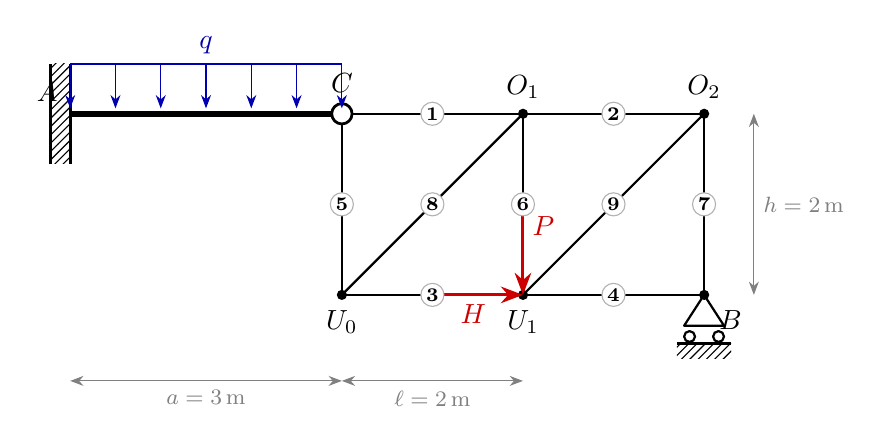
\begin{tikzpicture}[scale=1.15, >=Stealth, line join=round]
  \coordinate (A) at (0.000,0.000);
  \coordinate (C) at (3.000,0.000);
  \coordinate (O1) at (5.000,0.000);
  \coordinate (O2) at (7.000,0.000);
  \coordinate (U0) at (3.000,-2.000);
  \coordinate (U1) at (5.000,-2.000);
  \coordinate (U2) at (7.000,-2.000);
  \draw[thick] (C) -- (O1);
  \draw[thick] (O1) -- (O2);
  \draw[thick] (U0) -- (U1);
  \draw[thick] (U1) -- (U2);
  \draw[thick] (C) -- (U0);
  \draw[thick] (O1) -- (U1);
  \draw[thick] (O2) -- (U2);
  \draw[thick] (U0) -- (O1);
  \draw[thick] (U1) -- (O2);
  \draw[line width=2.2pt] (A) -- (C);
  \fill (C) circle (1.6pt);
  \fill (O1) circle (1.6pt);
  \fill (O2) circle (1.6pt);
  \fill (U0) circle (1.6pt);
  \fill (U1) circle (1.6pt);
  \fill (U2) circle (1.6pt);
  \draw[fill=white,line width=1pt] (C) circle (3.2pt);
  \draw[line width=1.1pt] (0.000,-0.550) -- (0.000,0.550);
  \fill[pattern=north east lines] (-0.220,-0.550) rectangle (0.000,0.550);
  \draw[line width=1.1pt] (-0.220,-0.550) -- (-0.220,0.550);
  \draw[thick] (7.000,-2.000) -- (6.780,-2.340) -- (7.220,-2.340) -- cycle;
  \draw[thick] (6.840,-2.460) circle (0.06) (7.160,-2.460) circle (0.06);
  \draw[line width=1.1pt] (6.700,-2.540) -- (7.300,-2.540);
  \fill[pattern=north east lines] (6.700,-2.700) rectangle (7.300,-2.540);
  \draw[blue!70!black,thick] (0.000,0.550) -- (3.000,0.550);
  \draw[->,blue!70!black] (0.000,0.550) -- (0.000,0.06);
  \draw[->,blue!70!black] (0.500,0.550) -- (0.500,0.06);
  \draw[->,blue!70!black] (1.000,0.550) -- (1.000,0.06);
  \draw[->,blue!70!black] (1.500,0.550) -- (1.500,0.06);
  \draw[->,blue!70!black] (2.000,0.550) -- (2.000,0.06);
  \draw[->,blue!70!black] (2.500,0.550) -- (2.500,0.06);
  \draw[->,blue!70!black] (3.000,0.550) -- (3.000,0.06);
  \node[blue!70!black,above] at (1.500,0.550) {$q$};
  \draw[->,red!80!black,line width=1.1pt] (5.000,-1.050) -- (5.000,-2.000);
  \node[red!80!black,above right] at (5.000,-1.450) {$P$};
  \draw[->,red!80!black,line width=1.1pt] (4.050,-2.000) -- (5.000,-2.000);
  \node[red!80!black,below] at (4.450,-2.000) {$H$};
  \node[circle,fill=white,draw=gray!60,inner sep=0.7pt,font=\scriptsize] at (4.000,0.000) {\textbf{1}};
  \node[circle,fill=white,draw=gray!60,inner sep=0.7pt,font=\scriptsize] at (6.000,0.000) {\textbf{2}};
  \node[circle,fill=white,draw=gray!60,inner sep=0.7pt,font=\scriptsize] at (4.000,-2.000) {\textbf{3}};
  \node[circle,fill=white,draw=gray!60,inner sep=0.7pt,font=\scriptsize] at (6.000,-2.000) {\textbf{4}};
  \node[circle,fill=white,draw=gray!60,inner sep=0.7pt,font=\scriptsize] at (3.000,-1.000) {\textbf{5}};
  \node[circle,fill=white,draw=gray!60,inner sep=0.7pt,font=\scriptsize] at (5.000,-1.000) {\textbf{6}};
  \node[circle,fill=white,draw=gray!60,inner sep=0.7pt,font=\scriptsize] at (7.000,-1.000) {\textbf{7}};
  \node[circle,fill=white,draw=gray!60,inner sep=0.7pt,font=\scriptsize] at (4.000,-1.000) {\textbf{8}};
  \node[circle,fill=white,draw=gray!60,inner sep=0.7pt,font=\scriptsize] at (6.000,-1.000) {\textbf{9}};
  \node[above left=1pt] at (A) {$A$};
  \node[above=4pt] at (C) {$C$};
  \node[above=2pt] at (O1) {$O_{1}$};
  \node[above=2pt] at (O2) {$O_{2}$};
  \node[below=2pt] at (U0) {$U_{0}$};
  \node[below=2pt] at (U1) {$U_{1}$};
  \node[below right=2pt] at (U2) {$B$};
  \draw[<->,gray] (0.000,-2.950) -- (3.000,-2.950) node[midway,below,font=\footnotesize]{$a=3$\,m};
  \draw[<->,gray] (3.000,-2.950) -- (5.000,-2.950) node[midway,below,font=\footnotesize]{$\ell=2$\,m};
  \draw[<->,gray] (7.550,0) -- (7.550,-2.000) node[midway,right,font=\footnotesize]{$h=2$\,m};
\end{tikzpicture}
\end{center}
\par\medskip\textbf{1.\ Static determinacy}\\[-2pt]
Counting criterion $n = r - (3 + v)$ with $r$ support reactions and $v$ hinge conditions:
\[ n = r - (3+v) = 4 - (3+1) = 0 \quad\Rightarrow\quad \text{the system is statically determinate.} \]
\par\medskip\textbf{2.\ Support reactions and hinge force}\\[-2pt]
$A_x = -5$\,kN,\quad $A_y = 30.5$\,kN,\quad $M_A = 64.5$\,kNm,\quad $B_y = 7.5$\,kN\\[2pt]$C_x = 5$\,kN,\quad $C_y = -12.5$\,kN\par
\par\medskip\textbf{3.\ Truss member forces}\par
\begin{center}\renewcommand{\arraystretch}{1.15}
\begin{tabular}{c r l}
\toprule
Member & Member force $S$ [kN] & Type \\
\midrule
  1 (C\,--\,O1) & 5 & tension \\
  2 (O1\,--\,O2) & -7.5 & compression \\
  3 (U0\,--\,U1) & 12.5 & tension \\
  4 (U1\,--\,U2) & 0 & zero-force \\
  5 (C\,--\,U0) & 12.5 & tension \\
  6 (O1\,--\,U1) & 12.5 & tension \\
  7 (O2\,--\,U2) & -7.5 & compression \\
  8 (U0\,--\,O1) & -17.68 & compression \\
  9 (U1\,--\,O2) & 10.61 & tension \\
\bottomrule
\end{tabular}\end{center}
\begin{center}
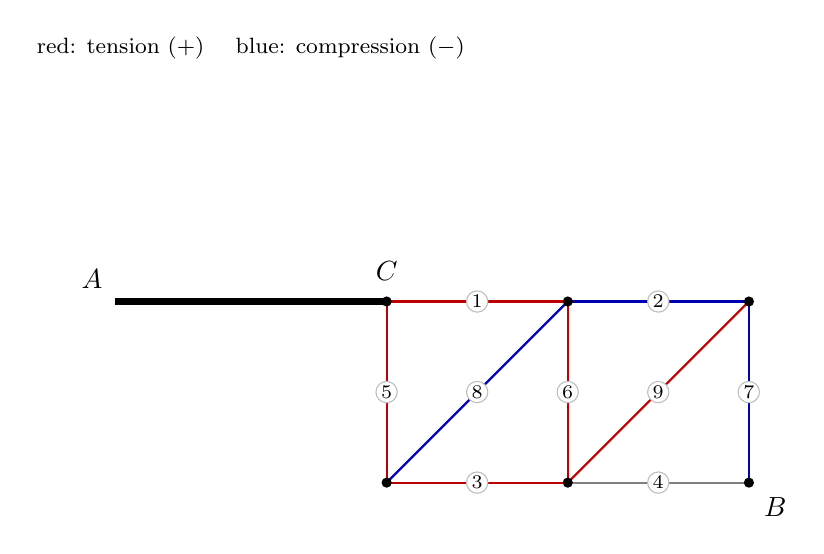
\begin{tikzpicture}[scale=1.15, >=Stealth, line join=round]
  \coordinate (A) at (0.000,0.000);
  \coordinate (C) at (3.000,0.000);
  \coordinate (O1) at (5.000,0.000);
  \coordinate (O2) at (7.000,0.000);
  \coordinate (U0) at (3.000,-2.000);
  \coordinate (U1) at (5.000,-2.000);
  \coordinate (U2) at (7.000,-2.000);
  \draw[thick,red!75!black] (C) -- (O1);
  \draw[thick,blue!70!black] (O1) -- (O2);
  \draw[thick,red!75!black] (U0) -- (U1);
  \draw[thick,gray] (U1) -- (U2);
  \draw[thick,red!75!black] (C) -- (U0);
  \draw[thick,red!75!black] (O1) -- (U1);
  \draw[thick,blue!70!black] (O2) -- (U2);
  \draw[thick,blue!70!black] (U0) -- (O1);
  \draw[thick,red!75!black] (U1) -- (O2);
  \draw[line width=2.2pt] (A) -- (C);
  \fill (C) circle (1.6pt);
  \fill (O1) circle (1.6pt);
  \fill (O2) circle (1.6pt);
  \fill (U0) circle (1.6pt);
  \fill (U1) circle (1.6pt);
  \fill (U2) circle (1.6pt);
  \node[circle,fill=white,draw=gray!50,inner sep=0.6pt,font=\scriptsize] at (4.000,0.000) {1};
  \node[circle,fill=white,draw=gray!50,inner sep=0.6pt,font=\scriptsize] at (6.000,0.000) {2};
  \node[circle,fill=white,draw=gray!50,inner sep=0.6pt,font=\scriptsize] at (4.000,-2.000) {3};
  \node[circle,fill=white,draw=gray!50,inner sep=0.6pt,font=\scriptsize] at (6.000,-2.000) {4};
  \node[circle,fill=white,draw=gray!50,inner sep=0.6pt,font=\scriptsize] at (3.000,-1.000) {5};
  \node[circle,fill=white,draw=gray!50,inner sep=0.6pt,font=\scriptsize] at (5.000,-1.000) {6};
  \node[circle,fill=white,draw=gray!50,inner sep=0.6pt,font=\scriptsize] at (7.000,-1.000) {7};
  \node[circle,fill=white,draw=gray!50,inner sep=0.6pt,font=\scriptsize] at (4.000,-1.000) {8};
  \node[circle,fill=white,draw=gray!50,inner sep=0.6pt,font=\scriptsize] at (6.000,-1.000) {9};
  \node[above left=1pt] at (A) {$A$};
  \node[above=4pt] at (C) {$C$};
  \node[below right=2pt] at (U2) {$B$};
  \node[font=\footnotesize,align=center] at (1.50,2.80) {red: tension $(+)$ \quad blue: compression $(-)$};
\end{tikzpicture}
\end{center}
\par\medskip\textbf{4.\ Section-force diagrams of the bending beam $A$--$C$}\par
\begin{center}
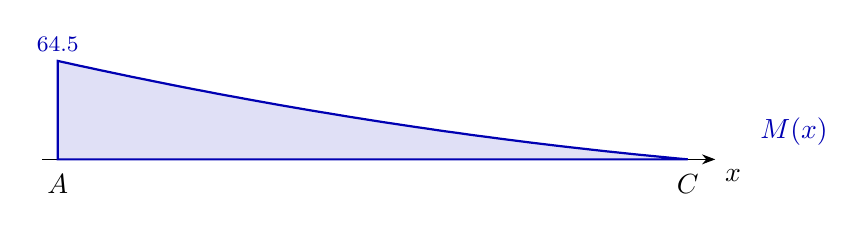
\begin{tikzpicture}[>=Stealth]
  \draw[->] (-0.2,0) -- (8.35,0) node[below right]{$x$};
  \node[below=2pt] at (0,0) {$A$};
  \node[below=2pt] at (8.00,0) {$C$};
  \filldraw[fill=blue!70!black!12,draw=blue!70!black,thick] (0,0) -- plot coordinates {(0.000,1.250) (0.133,1.221) (0.267,1.191) (0.400,1.163) (0.533,1.134) (0.667,1.106) (0.800,1.078) (0.933,1.050) (1.067,1.023) (1.200,0.996) (1.333,0.969) (1.467,0.942) (1.600,0.916) (1.733,0.890) (1.867,0.865) (2.000,0.839) (2.133,0.814) (2.267,0.790) (2.400,0.765) (2.533,0.741) (2.667,0.717) (2.800,0.693) (2.933,0.670) (3.067,0.647) (3.200,0.624) (3.333,0.602) (3.467,0.580) (3.600,0.558) (3.733,0.536) (3.867,0.515) (4.000,0.494) (4.133,0.473) (4.267,0.453) (4.400,0.433) (4.533,0.413) (4.667,0.394) (4.800,0.374) (4.933,0.355) (5.067,0.337) (5.200,0.318) (5.333,0.300) (5.467,0.283) (5.600,0.265) (5.733,0.248) (5.867,0.231) (6.000,0.214) (6.133,0.198) (6.267,0.182) (6.400,0.166) (6.533,0.151) (6.667,0.136) (6.800,0.121) (6.933,0.106) (7.067,0.092) (7.200,0.078) (7.333,0.064) (7.467,0.051) (7.600,0.038) (7.733,0.025) (7.867,0.012) (8.000,-0.000)} -- (8.000,0) -- cycle;
  \node[above,blue!70!black,font=\footnotesize] at (0.000,1.250) {64.5};
  \node[blue!70!black,right] at (8.80,0.35) {$M(x)$};
\end{tikzpicture}
\\[6pt]
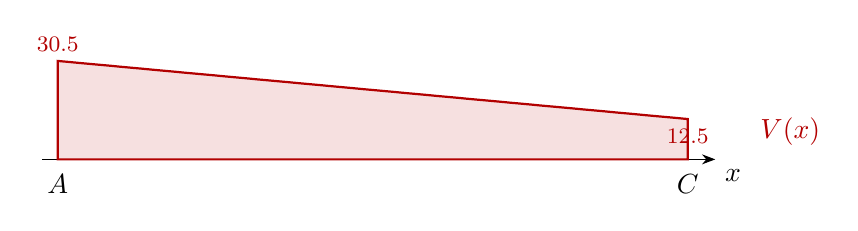
\begin{tikzpicture}[>=Stealth]
  \draw[->] (-0.2,0) -- (8.35,0) node[below right]{$x$};
  \node[below=2pt] at (0,0) {$A$};
  \node[below=2pt] at (8.00,0) {$C$};
  \filldraw[fill=red!70!black!12,draw=red!70!black,thick] (0,0) -- plot coordinates {(0.000,1.250) (0.133,1.238) (0.267,1.225) (0.400,1.213) (0.533,1.201) (0.667,1.189) (0.800,1.176) (0.933,1.164) (1.067,1.152) (1.200,1.139) (1.333,1.127) (1.467,1.115) (1.600,1.102) (1.733,1.090) (1.867,1.078) (2.000,1.066) (2.133,1.053) (2.267,1.041) (2.400,1.029) (2.533,1.016) (2.667,1.004) (2.800,0.992) (2.933,0.980) (3.067,0.967) (3.200,0.955) (3.333,0.943) (3.467,0.930) (3.600,0.918) (3.733,0.906) (3.867,0.893) (4.000,0.881) (4.133,0.869) (4.267,0.857) (4.400,0.844) (4.533,0.832) (4.667,0.820) (4.800,0.807) (4.933,0.795) (5.067,0.783) (5.200,0.770) (5.333,0.758) (5.467,0.746) (5.600,0.734) (5.733,0.721) (5.867,0.709) (6.000,0.697) (6.133,0.684) (6.267,0.672) (6.400,0.660) (6.533,0.648) (6.667,0.635) (6.800,0.623) (6.933,0.611) (7.067,0.598) (7.200,0.586) (7.333,0.574) (7.467,0.561) (7.600,0.549) (7.733,0.537) (7.867,0.525) (8.000,0.512)} -- (8.000,0) -- cycle;
  \node[above,red!70!black,font=\footnotesize] at (0.000,1.250) {30.5};
  \node[below,red!70!black,font=\footnotesize] at (8.000,0.512) {12.5};
  \node[red!70!black,right] at (8.80,0.35) {$V(x)$};
\end{tikzpicture}
\\[6pt]
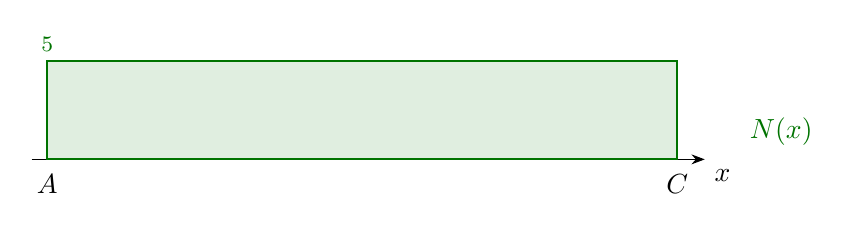
\begin{tikzpicture}[>=Stealth]
  \draw[->] (-0.2,0) -- (8.35,0) node[below right]{$x$};
  \node[below=2pt] at (0,0) {$A$};
  \node[below=2pt] at (8.00,0) {$C$};
  \filldraw[fill=green!45!black!12,draw=green!45!black,thick] (0,0) -- plot coordinates {(0.000,1.250) (0.133,1.250) (0.267,1.250) (0.400,1.250) (0.533,1.250) (0.667,1.250) (0.800,1.250) (0.933,1.250) (1.067,1.250) (1.200,1.250) (1.333,1.250) (1.467,1.250) (1.600,1.250) (1.733,1.250) (1.867,1.250) (2.000,1.250) (2.133,1.250) (2.267,1.250) (2.400,1.250) (2.533,1.250) (2.667,1.250) (2.800,1.250) (2.933,1.250) (3.067,1.250) (3.200,1.250) (3.333,1.250) (3.467,1.250) (3.600,1.250) (3.733,1.250) (3.867,1.250) (4.000,1.250) (4.133,1.250) (4.267,1.250) (4.400,1.250) (4.533,1.250) (4.667,1.250) (4.800,1.250) (4.933,1.250) (5.067,1.250) (5.200,1.250) (5.333,1.250) (5.467,1.250) (5.600,1.250) (5.733,1.250) (5.867,1.250) (6.000,1.250) (6.133,1.250) (6.267,1.250) (6.400,1.250) (6.533,1.250) (6.667,1.250) (6.800,1.250) (6.933,1.250) (7.067,1.250) (7.200,1.250) (7.333,1.250) (7.467,1.250) (7.600,1.250) (7.733,1.250) (7.867,1.250) (8.000,1.250)} -- (8.000,0) -- cycle;
  \node[above,green!45!black,font=\footnotesize] at (0.000,1.250) {5};
  \node[green!45!black,right] at (8.80,0.35) {$N(x)$};
\end{tikzpicture}
\end{center}
\end{document}